\documentclass[11pt, a4paper]{article}
 
\usepackage{amsmath, amssymb, amsthm, mathtools,pgfplots}
\usepackage{tikz}
\usepackage{pgfplots}
\usepackage{graphicx,caption,multicol}
\usepackage{verbatim}
%\usepackage{venndiagram}
\usepackage[cm]{fullpage}
\usepackage{color,enumerate,framed}
\usetikzlibrary{patterns}
%\captionsetup{labelformat=empty,labelsep=none}
\usepackage{mdwlist}
%\usepackage[nohug]{diagrams}
\usepackage[T1]{fontenc}

\usepackage[margin=1in]{geometry} 
\usepackage{natbib}
\usepackage{hyperref}

\title{
	\vspace*{-1.5cm}
	\scshape 40.752 Algorithmic Game Theory\\
	\vspace{0.5cm}
	Project Proposal\\
	\vspace{0.5cm}
	{\bfseries\Large TO COOPERATE OR TO COMPETE: \\
		A GAME THEORETIC MODEL}\\
	\vspace{0.5cm}}

\author{Lai Zhangsheng \qquad \qquad Nguyen Tan Thai Hung}
\date{\today}

\begin{document}

\maketitle
\bibliographystyle{apalike}

\section{Motivation}
The idea for this project is drawn upon our own observation from past work experiences. 

In the workplace, managers typically want their staff to cooperate in order to achieve a good performance for the department. However, staff appraisals are done according to a bell curve, which disincentify people to cooperate (If I help you, you'll get better and my chance of getting the top post is less). This appraisal mechanism is thus not incentive compatible. 

In the school context, we observe a similar phenomenon. Students should study together and help each other, but the bell curve system can cause competition among students, leading to inefficiency.

\section{Project description}
In this project, we want to model what happens in the workplace from a game theoretic perspective. Then, we will attempt to figure out a way to quantify the performance, and propose a better mechanism.

\subsection{The model}
For the simplest case, we will model the game as a two-agent payoff-maximizing game. The payoff each agent receives depend on whether his performance is better than the other agent. Each agent's performance depends on whether they perform their task alone or with help from the other agent. We believe that under the ranking-base reward scheme, the equilibrium strategy is for each agent to work alone, whereas the socially optimal strategy is for them to cooperate. We will then compute the Price of Anarchy and its bounds.

\subsection{Mechanism design}
After determining the performance of the existing reward scheme, we will attempt to propose a different reward scheme such that cooperation becomes the dominant strategy. We draw our inspiration from real life games such as World of Warcraft and DOTA, where we have seen cooperative efforts to achieve the game objectives. Hence, we hope to transfer what was applied in the games to the workplace setting.

\section{Experiment}
This may be somewhat too ambitious, but we hope to conduct an experimental game on the \href{http://arenalabs.co/}{ArenaLabs} website to verify our model.

\section{Theoretical background}
The problem was first mentioned in literature by \cite{Drago1991}. Since this seminal work, several scholars have investigated the problems in deeper details:
\begin{itemize}
	\item \cite{Drago1998} and \cite{Kistruck2016} discuss different reward structures to encourage cooperation.
	\item \cite{Banerjee2014} and \cite{Chakravarti2015} also explore incentive schemes, but with focus on knowledge sharing among researchers and team members.
	\item \cite{Immorlica2011} discussed a dueling game and show how bad head-on competition can get.
	\item \cite{Landers2015} described an interesting gamification experiment to understand how people actually behave when the reward mechanism is changed.
	
\end{itemize}
 
\section{Comparison with Prisoners' Dilemma}
The Prisoners' Dilemma's payoff table is 
\begin{table}[h]
	\centering
	\caption{Prisoners' Dilemma's payoff table}
	\begin{tabular}{c c c}
		        & Silent & Betray \\
		Silent  & 1, 1    & 3, 0     \\
		Betray  & 0, 3    & 2, 2
	\end{tabular}
\end{table}

The payoff table of our game is still to be determined, but we believe that there are some differences, and we may want to tackle some or all of them
\begin{itemize}
	\item In the Prisoners' Dilemma game, players can move only once and they are not allowed to talk to each other. In our game, both these constraints are not present.
	\item The Prisoners' Dilemma is symmetric, while it is reasonable to assume that our two office workers are different in many ways. For example, they have different skill sets.
\end{itemize}
\begin{table}[h]
	\centering
	\caption{Workplace game's payoff table}
	\begin{tabular}{c c c}
		          & Cooperate & Compete \\
		Cooperate & ?, ?      & ?, ?    \\
		 Compete  & ?, ?      & ?, ?
	\end{tabular}
\end{table}

\newpage

\section{The Model}
We shall consider an office game where there are $k$ agents, each with its own project. Every agent is assumed to have:
\begin{itemize}
\item the same time budget $T$
\item a daily schedule represented by a vector $t_i=(t_{i1},t_{i2},\ldots,t_{ik})$ with $\sum_{k}t_{ik}=T$.
\end{itemize}

For each project which is owned by a sole agent, there is a work output (performance) associated with it that is dependent on the total time (effort) invested into the project
\begin{align*}
p_j = \beta_j\log\left(t_{ii}+\sum_{i\neq j}^{k}\alpha_{ij}t_{ij}\right)
\end{align*}
where $\alpha_{ij}$ is the effectiveness (skill) if agent $i$ when working on project $j$ (w.r.t the owner) and $\beta_{j}$ is the value of the project. Here the $\log$ function is used to model the scenario when many agents choose to allocate their time to a particular project;  the work output will reach saturation over time, see Fig. \ref{fig:log}.


Using the performance $p_j$, we can assign a rank to each agent and then derive its corresponding payoffs:
\begin{align*}
u_j=f(r_j)\cdot g(P)
\end{align*}
where $P=\sum_{i}p_i$. The utility you derive depends on how well you perform relative to the other agents and how the company performs as a whole. 


\begin{figure}
\centering
\begin{tikzpicture}
\begin{axis}[scale=0.75,
  no markers,  domain=-8:12, samples=100,
   axis y line=center,
      axis x line=center,
   xlabel=$x$, ylabel=$y$,
  every axis y label/.style={at=(current axis.above origin),anchor=south},
  every axis x label/.style={at=(current axis.right of origin),anchor=west},
  height=8cm, width=12cm,
  enlargelimits=true, 
  clip=false,
  axis equal,
  xtick=\empty,
  ytick=\empty,
  ymin=-4,
 % ymax=4,
 xmin=-4,
  xmax=4,
  %axis equal
%  minor tick num =5
  ]
    \addplot[mark=none,smooth,color=red,thick,domain=-8:4] {1.7^x} node[pos=0.75,pin=120:{\color{black}$y=a^x$},inner sep=0pt] {};
 \addplot[mark=none,smooth,color=blue,thick] {ln(x)/ln(1.7)} node[pos=0.95,pin=-15:{\color{black}$y=\log_ax$},inner sep=0pt] {};
 \addplot[thick,dashed,domain=-4:8] {x} node[pos=0.95,pin=45:{\color{black}$y=x$},inner sep=0pt] {};
   \end{axis}
\end{tikzpicture}
\caption{Diminishing returns}\label{fig:log}
\end{figure}


\section{Discussion}
Further ideas on how we could model this problem was to think of it in the form of an atomic routing game. The time budget could be though of as the commodity of an agent and the agent needs to route all its commodity through a single source and sink network with parallel links. Each edge linking the source and sink represents a project and when an agent chooses to route some `flow' through a particular edge, it is just same as saying that the agent is investing time into that project. This may be extended to a larger network 


\begin{figure}[h]
\centering

\def\layersep{2.5cm}

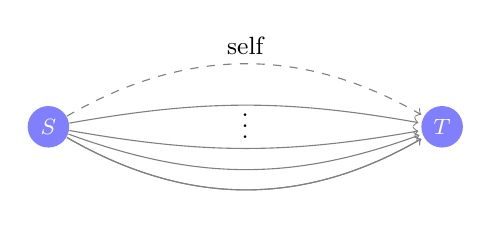
\begin{tikzpicture}[scale = 1,shorten >=1pt,->,draw=black!50, node distance=\layersep]
    \tikzstyle{every pin edge}=[<-,shorten <=1pt]
    \tikzstyle{neuron}=[circle,fill=black!25,minimum size=15pt,inner sep=0pt]
    \tikzstyle{output neuron}=[neuron, fill=red!50];
    \tikzstyle{n}=[neuron, fill=blue!50];

\node[n] (a) at (0,0) {\color{white}{\footnotesize $S$}};
\node[n] (b) at (5,0) {\color{white}{\footnotesize $T$}};
\draw (a) edge[bend left, dashed] node[above] {\small self } (b);
\draw (a) edge[bend right=-10] node[above] {\small } (b);

\draw (a) edge[bend right=10] node[above] {\small $\vdots$} (b);
\draw (a) edge[bend left=-20] node[above] {\small } (b);
\draw (a) edge[bend left=-30] node[above] {\small } (b);
\draw (a) edge[bend right] node[below] {\small } (b);
\end{tikzpicture}
\caption{Further ideas}\label{fig:}
\end{figure}

\bibliography{AGT_project}

\end{document}
